\documentclass[tikz,border=10pt]{standalone}
\usetikzlibrary{calc}
\newcommand{\n}{\sffamily\Large node n}
\newcommand{\invis}{\phantom{\sffamily\Large node n}}
\begin{document}
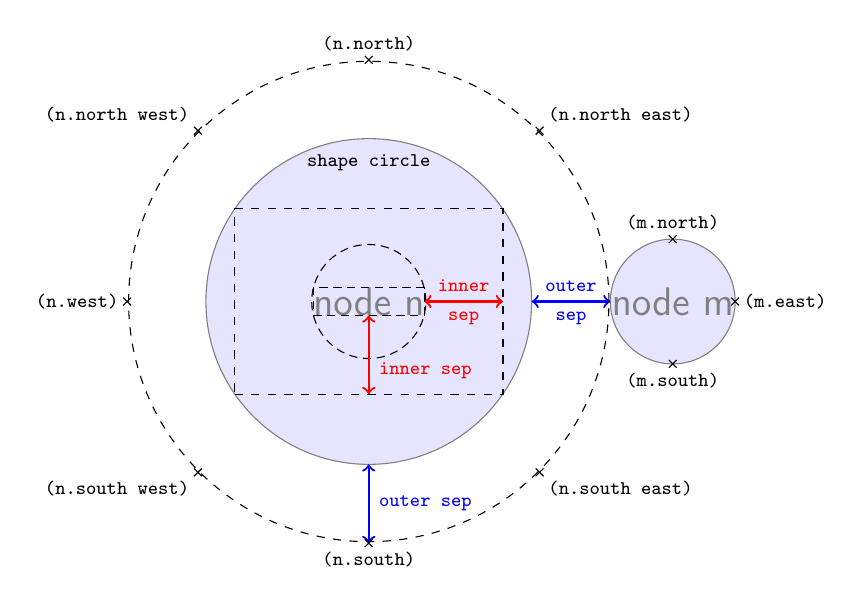
\begin{tikzpicture}[font={\scriptsize\ttfamily}]
% node n
\node[draw,circle,outer sep=1cm,inner sep=1cm,color=black!50, draw, fill=blue!10] (n) {{\n}};
% label "shape circle"
\node[above] at ($(n.center)!0.5!(n.north)$) {shape circle};

% dashed helper nodes with same position and (invisible) same text
\node[circle,draw,densely dashed,inner sep=0pt,outer sep=0pt] at (n.center) {\invis};
\node[rectangle,draw,densely dashed,inner sep=0pt,outer sep=0pt] at (n.center) {\invis};
\node (o) [rectangle,draw, dashed,inner sep=1cm,outer sep=0pt] at (n.center) {\invis};

% neighbor node
\node[circle,inner sep=0,outer sep=0,draw,right,color=black!50, draw, fill=blue!10] 
    (m) at(n.east) {{\sffamily\Large node m}};

% vertical sep
\draw[<->,thick,blue] (n.south)
  --++(0,1cm) node[midway,right]{outer sep};
\draw[<->,thick,red] (o.south)
  -- ++(0,1cm) node[pos=0.3,right]{inner sep};

% horizontal sep
\draw[<->,red,thick] (o.east) -- ++(-1cm,0)
  node[midway,above] {inner} node[midway,below] {sep};
\draw[<->,blue,thick] (m.west) -- ++(-1cm,0)
  node[midway,above] {outer} node[midway,below] {sep};

% some anchors
\foreach \anchor/\placement in
  {south west/below left,south/below,north/above,north west/above left,
     north east/above right,south east/below right,west/left}
     \draw[shift=(n.\anchor)] plot[mark=x] coordinates{(0,0)}
      node[\placement,label distance = 0mm,inner sep=3pt] {(n.\anchor)};
\foreach \anchor/\placement in
  {east/right,south/below,north/above}
     \draw[shift=(m.\anchor)] plot[mark=x] coordinates{(0,0)}
      node[\placement,label distance = 0mm,inner sep=3pt] {(m.\anchor)};

% random circle :-)
\draw[dashed] (n.center) circle (3.05cm);

\end{tikzpicture}
\end{document}
